\documentclass[../Thesis.tex]{subfiles}
\graphicspath{{\subfix{../figures/}}}
% \epstopdfsetup{outdir={../figures/}}
\begin{document}

\chapter{Method}

\section{Copula based network discovery}
Suppose a set of random variables $(X_i)$ is given. The method presented in this section aims to discover direct relationships between pairs $X_i$ and $X_j$ for $i\neq j$. These relationships can be presented using an undirected graph. We will later discuss methods of directing edges such that a causal network may be discovered.

One way of discovering such a network from a set of observations is through mutual information. Namely, suppose that we have obtained a matrix $G_{obs}$ with similarities between each pair of random variables. We will use mutual information as similarity. Let $G_{dir}$ be the information on each edge of the graph i.e. only the direct effects between pairs of variables.
$$G_{obs} = G_{dir} + G_{indir} = G_{dir} + G_{dir}^2 + G_{dir}^3 + \dots = \left(I - G_{dir}\right)^{-1} - I = G_{dir} \left(I - G_{dir}\right)^{-1}$$
where it is assumed that the above infinite sum converges. A necessary and sufficient condition for this is that $\rho \left(G_dir\right) < 1$ where $\rho\left( \cdot \right)$ denotes the spectral radius.

It follows that $G_{dir}$ can be calculated as
$$G_{dir} = G_{obs} \left(I + G_{obs}\right)^{-1}$$
Furthermore, as described by ... . As $G_{obs}$ is symmetric it is diagonalizable with a matrix $U$ such that $\Lambda_{obs} = U^T G_{obs} U$ where $\Lambda_{obs}$ is a diagonal matrix containing the spectral values with multiplicity in any ordering. It follows that since $\rho\left(G_{obs}\right) < 1$, $\lambda_{obs} + I$ is also invertible and
$$G_{dir} = U \Lambda_{dir} U^T$$
Where $\Lambda_{dir} = \Lambda_{obs} \left(I + \Lambda_{obs}\right)^{-1}$ i.e. $\left[\Lambda_{dir}\right]_{ii} = \frac{\lambda_{obs}}{1 + \lambda_{obs}}$ and $0$ elsewhere. Whether this is better than a normal inversion of $I + G_{obs}$ is at this point unknown.

At this point, we only need $G_{obs}$ and as mentioned earlier we will use mutual information. However, to make the calculations more robust and efficient we will use a closely related measure of dependence, namely CE which is defined as follows
$$ CE\left(X_1,\dots, X_n\right) = -\int \dots \int_{[0,1]^n} c\left(u_1,\dots, u_n\right) \log_{b}c\left(u_1,\dots, u_n\right) \, d u_1 \dots d u_n$$
where $c(\cdot)$ is the uniquely defined copula of the joint distribution $f_{\mathbf{X}}(\cdot)$. We show that the above is indeed equal to the negative mutual information. First, we realize that from definition,
\begin{align*}
    c(u_1,\dots , u_n) & = \partial_{\mathbf{u}} C(u_1,\dots,u_n)                                                        \\
                       & = \partial_{\mathbf{u}} F\left(F_1^{-1}\left(u_1\right), \dots, F_n^{-1}\left(u_n\right)\right) \\
                       & = f\left(x_1,\dots, x_n\right) \frac{1}{f_1(x_1)\dots f_n(x_n)}
\end{align*}
Thus
\begin{align*}
    -CE & = \int\dots \int_{[0,1]^n} c\left(u_1,\dots, u_n\right) \log c\left(u_1\dots,u_n\right) \, d u_1, \dots, d u_n                                                                               \\
        & =\int\dots \int_{[0,1]^n} c\left(u_1,\dots, u_n\right) \log c\left(u_1\dots,u_n\right) \, d F_1(x_1), \dots, d F_n(x_n)                                                                      \\
        & = \int \dots \int_{\mathbb{R}^n} \frac{f(x_1,\dots, x_n)}{f_1(x_1)\dots f_n(x_n)} \log\left(\frac{f(x_1,\dots, x_n)}{f_1(x_1)\dots f_n(x_n)}\right) f_1(x_1)\dots f_n(x_n) \, dx_1\dots dx_n \\
        & = \int \dots \int_{\mathbb{R}^n} f(x_1,\dots, x_n) \log\left(\frac{f(x_1,\dots, x_n)}{f_1(x_1)\dots f_n(x_n)}\right)  \, dx_1\dots dx_n                                                      \\
        & = MI
\end{align*}
Hence, we obtain $G_{obs}$ from the pairwise copula entropy (CE)
$$G_{obs} = \begin{bmatrix}
        0        & - CE_{12} & \dots  & - CE_{1n} \\
        -CE_{21} & 0         & \dots  & - CE_{2n} \\
        \vdots   & \vdots    & \ddots & \vdots    \\
        -CE_{n1} & -CE_{n2}  & \dots  & 0
    \end{bmatrix}$$

Although theoretically $-NCE_{ii} = \infty$ for all $i$, we put $0$ in the diagonal because we do not want self explanation as these are trivial. The argument for calculating CE instead of MI are due to the finite volume integral and simpler integrand. In particular, using the copulas, we avoid the fraction $\frac{f(x_1,\dots,x_n)}{f_1(x_1)\dots f_n(x_n)}$ which could easily result in numerical instability e.g. when both $f$ and $f_i$s are close to 0.

Finally, from the deconvoluted information matrix $D_{dir}$ we may choose a threshold $t$ for choosing which edges are significant. The choice of $t$


\newpage
\begin{theorem}[Sklar's theorem] \label{thm: Sklar}
    For a random vector $\boldsymbol X$ with CDF $F$ and univariate marginal CDFs $F_1, \dots, F_d$. There exists a copula $C$ such that
    $$ F(x_1,\dots,x_d) = C(F_1(x_1), \dots, F_d(x_d)) $$
    If $X$ is continuous, $C$ is unique.
\end{theorem}

The following corollary follows immediately
\begin{corollary} \label{coro: Coordinate transformation}
    Coordinate transformation

    Under the assumptions of \autoref{thm: Sklar}, given any set $(T_1, \dots, T_d)$ of strictly increasing functions, if $C$ is a copula of $(X_1,\dots, X_d)$ then it is also a copula of $(T_1(X_1), \dots, T_d(X_d))$.
\end{corollary}

\begin{proof}
    Suppose $(X_1 , \dots , X_d)$ permits a copula $C$ and let $T_i$ be given as stated. Consider coordinate wise the result of the transformation $Y_i = T_i(X_i)$ and consider the CDF $F_{Y_i}(y_i)$
    $$F_{Y_i}(y_i) = \mathbb{P}\left(Y_i \leq y_i\right) = \mathbb{P}\left(T_i^{-1}(Y_i) \leq T_i^{-1}(y_i)\right) = \mathbb{P}\left(X_i \leq x_i\right) = F_{X_i}(x_i)$$
    Thus
    \begin{align*}
        F_{\boldsymbol X} (x_1,\dots , x_d) & = C\left( F_{X_1}(x_1), \dots, F_{X_d}(x_d)\right) \\
                                            & = C\left( F_{Y_1}(y_1), \dots, F_{Y_d}(y_d)\right) \\
                                            & = F_{\boldsymbol Y}(y_1, \dots, y_d)
    \end{align*}
    where Sklar's theorem have been used for the final equality.
\end{proof}

The above corollary is actually equivalent with a seemingly stronger statement and follows easily
\begin{proposition}
    Since $T_i$ is strictly increasing, the inverse $T_i^{-1}$ exists and is also strictly increasing. Thus, the above implication is bidirectional and hence for strictly increasing functions $T_i$, $C$ is a copula of $\left(X_1,\dots,X_d\right)$ if and only if it is a copula of $\left(T_1(X_1),\dots, T_d(X_d)\right)$.
\end{proposition}




\newpage
\section{Algorithms}
\begin{algorithm}[H]
    \caption{$G_{obs}$ computation}\label{alg:Gobs1}
    \begin{algorithmic}
        \Require $N > 0$             \Comment{Number of variables}
        % \Ensure $y = x^n$
        % \State $y \gets 1$
        % \State $X \gets x$
        % \State $N \gets n$
        \For{$1\leq i < j \leq N$}
        \State Estimate $F_i$ and $F_j$ from $x_i^{\mathcal{D}}$ and $x_j^{\mathcal{D}}$
        \State $u_i^{\mathcal{D}} \gets F_i(x_i^{\mathcal{D}})$
        \State $u_j^{\mathcal{D}} \gets F_j(x_j^{\mathcal{D}})$
        \State Estimate $C_{ij}$ from $u_i^{\mathcal{D}}$ and $u_j^{\mathcal{D}}$
        \State Compute $NCE_{ij}$
        \State $G_{ij}, G_{ji} \gets -NCE_{ij}$
        \EndFor
    \end{algorithmic}
\end{algorithm}



\begin{algorithm}
    \caption{(ND) Network Deconvolution}\label{alg:ND}
    \begin{algorithmic}
        \Require $G_{obs}$             \Comment{Input observational matrix}
        % \For{$0\leq i < j < N$}
        \State $\left[G_{obs}\right]_{ii} \gets 0, \; \forall 1\leq i \leq N$                    \Comment{zero-diagonal}
        \State $Q_p \gets G_{[1-\alpha]}$
        \State Set $G_{obs}$ 0, where $G_{obs} < Q_p$
        \State Compute eigendecomposition $Q,\Lambda$ of $G_{obs}$
        \State $\lambda^+ \gets  \max{ \left( \lambda^{\text{max}},0 \right) }$
        \State $\lambda^- \gets -\min{ \left( \lambda^{\text{min}},0 \right) }$
        \State $m^+ \gets \frac{1-\beta}{\beta} \lambda^+$
        \State $m^- \gets \frac{1+\beta}{\beta} \lambda^-$
        \State $m \gets \max{\left( m^+, m^- \right)}$
        \State $\hat{\Lambda} \gets \Lambda \left(mI + \Lambda\right)^{-1}$
        \State \Return $Q \hat{\Lambda} Q^T$
        % \EndFor
    \end{algorithmic}
\end{algorithm}

\begin{remark}
    The $1-\alpha$ quantile, denoted by $G_{[1-alpha]}$ (of the upper triangular matrix), can be computed in many ways. As it is only used to filter the $G_{obs}$ matrix, its precise value does not matter. Only the property $\alpha$ part of the observations are below $Q_{1-\alpha}$ and $1-\alpha$ are above (or equal to) $Q_{1-\alpha}$. This property is for example fulfilled by the quantile function \texttt{quantile} from \texttt{NumPy} (v. 1.26.4). Thus setting $\alpha = 1$ will result in $G_{obs}$ retaining all entries (except for the diagonal entries).
\end{remark}

\begin{remark}
    The $\beta \in (0,1)$ parameter serves as a sort of regularization. The algorithm above also maps the maximum absolute value of the eigenvalues (the spectral radius) to $\beta$ as is also pointed out in the implementation of \textcolor{red}{Source code from Nature paper at https://compbio.mit.edu/nd/index.html}. The proof of this is shown below
\end{remark}

\begin{proof}
    To show that eigenvalues i.e. the diagonal elements of $\Lambda$ resulting from \autoref{alg:ND} all fall in the interval $[-\beta, \beta]$ (i.e. $\sigma\left(Q \Lambda Q^T\right) \subseteq [-\beta, \beta]$) where at least one $\lambda$ is mapped to either $-\beta$ or $\beta$, first notice that clearly the resulting eigenvalues of $G_{dir} = Q \hat{\Lambda} Q^T$ are clearly given by $\frac{\lambda_i}{m + \lambda_i}$ where $(\lambda_i)_{\{1,\dots, N\}}$ are the (real) eigenvalues of $G_{obs}$ from the definition of $\hat{\Lambda}$. We will show the above by first considering $\lambda \geq 0$ and $\lambda < 0$.

    For $\lambda \geq 0$, clearly $m \geq \frac{1-\beta}{\beta} \lambda^+$, thus
    $$\frac{\lambda}{m + \lambda} = \frac{1}{1 + m/\lambda} \leq \frac{1}{1 + \frac{\lambda^+}{\lambda} \frac{1-\beta}{\beta}} \leq \frac{1}{1 + \frac{1-\beta}{\beta}} = \beta$$
    where the final inequality follows from $\lambda \leq \lambda^+$. Hence $[0,\lambda^+] \to [0, \beta]$.

    Furthermore, for $0 > \lambda \geq -\lambda^- $, note that also $m \geq \frac{1+\beta}{\beta} \lambda^-$. Since $\beta \in (0,1]$, $m + \lambda \geq \frac{1 + \beta}{\beta} \lambda^- + \lambda> 0$ and thus $\frac{\lambda}{m + \lambda} < 0$ which implies
        $$- \frac{\lambda}{m + \lambda} \leq  \frac{- \lambda}{\frac{1 + \beta}{\beta}\lambda^- + \lambda} = \frac{1}{\frac{1+ \beta}{\beta} \frac{\lambda^-}{-\lambda} - 1} \leq \frac{1}{ \frac{1+\beta}{\beta} - 1} = \beta$$
        i.e. $[-\lambda^-,0) \to [-\beta, 0)$. This shows that indeed all the eigenvalues of $G_{dir}$ is numerically less that or equal to $\beta$. Finally, assuming $m\neq 0$ or equivalently that $G_{obs} \neq \mathbf{0}$, either $m = \frac{1-\beta}{\beta}\lambda^+$ (and thus $\lambda^+ \neq 0$ is an eigenvalue of $G_{obs}$) for which the above shows that indeed $\lambda^+$ is mapped to $\beta$ or $m = \frac{1+\beta}{\beta} \lambda^-$ (and hence $\lambda^- \neq 0$ and thus $-\lambda^-$ is an eigenvalue of $G_{obs}$) for which $-\lambda^-$ is mapped to $-\beta$. This shows that $G_dir$ indeed has an eigenvalue which numerical value is $\beta$.
\end{proof}



\newpage
\section{Examples}
In this section, we will investigate how the algorithms \autoref{alg:Gobs1} and \autoref{alg:ND} works in junction and, if so, observe how the algorithm can fail and what may be done to correct such cases. Initially, a few simple examples involving exponentiated multivariate Gaussians $\boldsymbol Y $.

\begin{example} \label{ex:1}
    Exponentiated multivariate Gaussian

    Let us consider a simple case with $\mathbf{Y} = e^{\mathbf{X}}$ (element wise exponentiation) where $X \sim \mathcal{N}\left(\mathbf{0}, \Sigma\right)$ where
    $$\Sigma = \begin{bmatrix}
            \sigma_1^2           & 0.9\sigma_1\sigma_2 & 0          \\
            0.9 \sigma_1\sigma_2 & \sigma_2^2          & 0          \\
            0                    & 0                   & \sigma_3^2
        \end{bmatrix}$$
    It is clear that to \autoref{alg:Gobs1}, the mean is non-important as simply corresponds to a scaling of the $Y_i$ variables. Furthermore, because of \autoref{coro: Coordinate transformation}, theoretically, due to the uniqueness of the Copula $C$ (as $\boldsymbol Y$ is continuous) we should expect near equal or very similar results for $\boldsymbol Y$ and $\boldsymbol X$ from \autoref{alg:Gobs1}. Additionally, different $\sigma$ corresponds to different scaling of $\boldsymbol X$, and thus we should observe equal or near equal $G_{dir}$ for all $\boldsymbol Y$. Initially, we shall see how this hypothesis holds up to the following three examples
    $$
        \boldsymbol\sigma = (0.07, 0.3, 0.9), \quad
        \boldsymbol\sigma = (1,1,1), \quad
        \boldsymbol\sigma = (1,2,3)
    $$
    In order for the sample size to not influence the results, we simulate a generous number of samples, namely, for the following results we have used $n = 10{,}000$ samples. For $\boldsymbol\sigma = (1,1,1)$, \autoref{alg:Gobs1} and \autoref{alg:ND} returns the following (using $\alpha = 1$ and $\beta = 0.99$)
    \begin{equation} \label{eq:s medium G_dir}
        G_{dir} =
        \begin{bmatrix}
            -0.33396 & 0.6660  & 0.02512    \\
            0.6660   & -0.3341 & 0.02730    \\
            0.02512  & 0.02730 & -0.0020583
        \end{bmatrix}
    \end{equation}
    Similarly, for $\boldsymbol\sigma = (0.07, 0.3, 0.9)$:
    \begin{equation} \label{eq:s small G_dir}
        G_{dir} =
        \begin{bmatrix}
            -0.3335 & 0.6665  & 0.01414     \\
            0.6665  & -0.3335 & 0.01418     \\
            0.01414 & 0.01418 & -0.00060124
        \end{bmatrix}
    \end{equation}
    Finally, for $\boldsymbol\sigma = (1,2,3)$:
    $$ G_{dir} =
        \begin{bmatrix}
            -0.1490 & 0.09535 & 0.3599  \\
            0.09535 & -0.2989 & 0.5831  \\
            0.3599  & 0.5831  & -0.4037
        \end{bmatrix}
    $$
    For $\boldsymbol\sigma = (1,1,1)$ and $\boldsymbol\sigma = (0.07, 0.3, 0.9)$ we observe the most resemblance to the $\Sigma$, although the resulting $G_{dir}$ deviate in the final column. The difference is likely produced by \autoref{alg:Gobs1} as if the resulting $G_{obs}$ was the same, then so would $G_{dir}$ and from the above argument, we know that theoretically this should be the case. For the final example, $\boldsymbol\sigma = (1,2,3)$, we see a completely different result and immediately suspect that there must be some numerical errors. Investigating the partial results of \autoref{alg:Gobs1} we immediately see a flaw in the supposedly uniform variables $U_i$ as shown in figure \autoref{fig:Gaussian 3x3 large s uniforms}
    \begin{figure}[H]
        \centering
        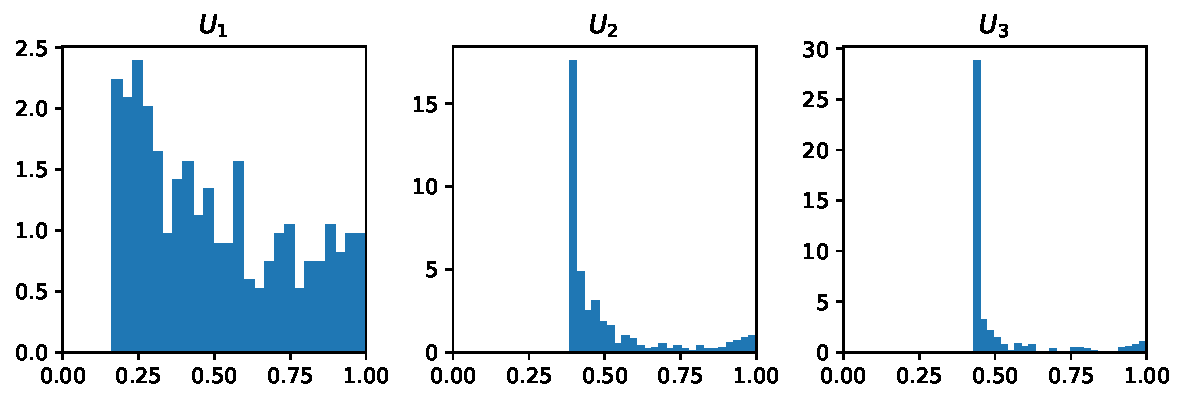
\includegraphics[width=0.99\linewidth]{figures/ND examples/Gaussian 3x3 large s uniforms.pdf}
        \caption{The samples transformed using $U_i = F_i(X_i)$ for $\boldsymbol\sigma = (1,2,3)$. These should be uniformly distributed, but clearly this is not the case for $U_2$ and $U_3$. Even $U_1$ does not quite resemble $10{,}000$ samples from a uniform distribution.}
        \label{fig:Gaussian 3x3 large s uniforms}
    \end{figure}
    Before handling this, the non-uniformity of $U_1$ in \autoref{fig:Gaussian 3x3 large s uniforms} is likely also present in the case when $\boldsymbol\sigma = (1,1,1)$. Indeed, \autoref{fig:Gaussian 3x3 medium s uniforms} shows that this is indeed the case.
    \begin{figure}[H]
        \centering
        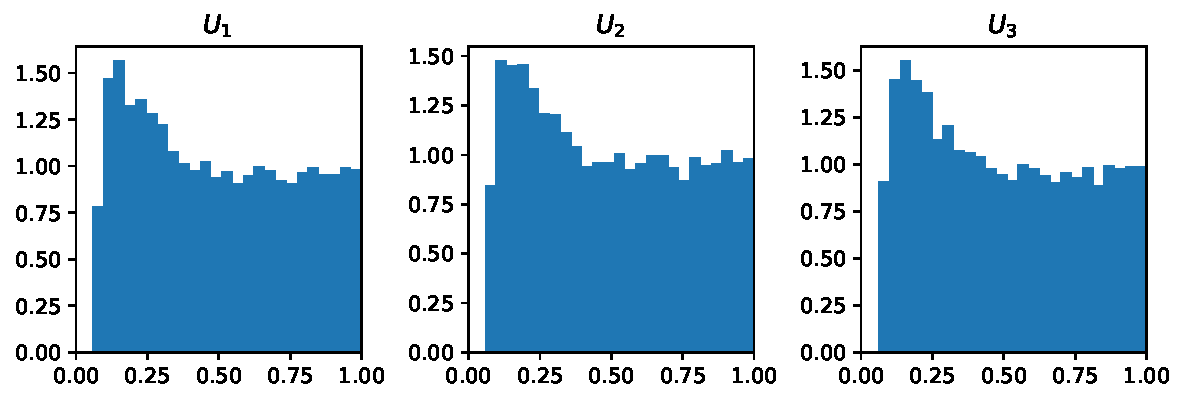
\includegraphics[width=0.99\linewidth]{figures/ND examples/Gaussian 3x3 medium s uniforms.pdf}
        \caption{The samples transformed using $U_i = F_i(X_i)$ for $\boldsymbol\sigma = (1,1,1)$.}
        \label{fig:Gaussian 3x3 medium s uniforms}
    \end{figure}
    Finally, just to be sure, $\boldsymbol\sigma = (0.07, 0.3, 0.9)$ is also shown in \autoref{fig:Gaussian 3x3 small s uniforms} and seems very reasonable, except for $U_3$.
    \begin{figure}[H]
        \centering
        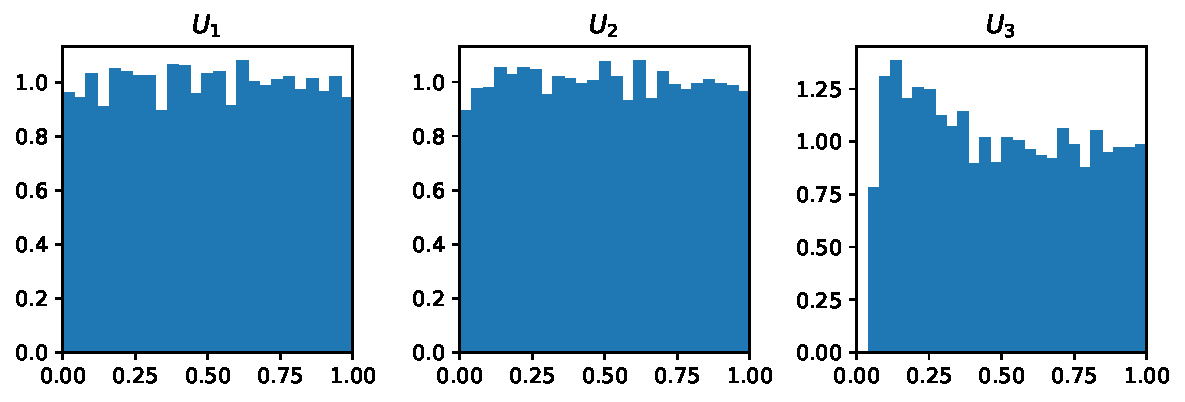
\includegraphics[width=0.99\linewidth]{figures/ND examples/Gaussian 3x3 small s uniforms.pdf}
        \caption{\raggedright The samples transformed using $U_i = F_i(X_i)$ for $\boldsymbol\sigma = (0.07, 0.3, 0.9)$.\hfill}
        \label{fig:Gaussian 3x3 small s uniforms}
    \end{figure}
    From the above examples, it seems that the larger the variance, the worse the uniforms turn out. Reasons for this could include numerical issues when trying to calculate $u_i^{(j)}$ form $y_i^{(j)}$ by $u_i^{(j)} = \int_{-\infty}^{y_i^{(j)}} f_i(y) \, dy$ and bad fitting of the kernel density estimate from observations. In particular, for values similar, which happens in the case for large $\sigma$ such that we observe large negative realizations of $X_i$, $y_i^{(j)}$ are almost 0, and when computing the integral could result in identical values. Furthermore, from \autoref{fig:Gaussian 3x3 large s X3 KDE} we see that indeed the fit is quite poor. Note that we have zoomed in on the interval $[-200 , 200]$ which contains $96.2\%$ of observations. The poor fit is primarily due to the use of Scott's Rule \textcolor{red}{as discussed above} which in this case overshoots the optimal bandwidth by a lot.
    \begin{figure}[H]
        \centering
        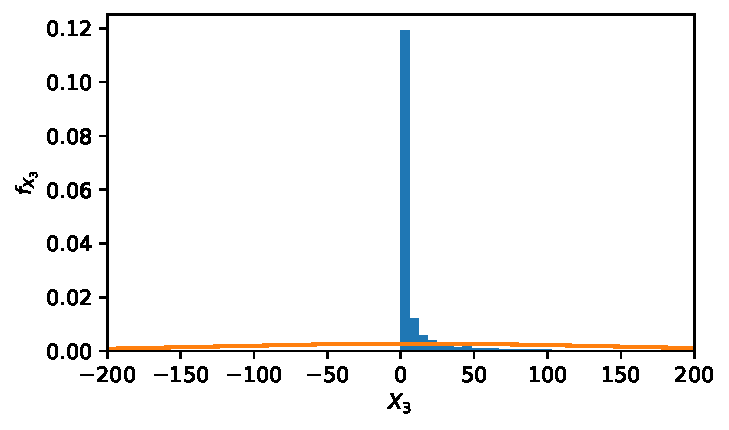
\includegraphics[width=0.7\linewidth]{figures/ND examples/Gaussian 3x3 large s X3 KDE.pdf}
        \caption{}
        \label{fig:Gaussian 3x3 large s X3 KDE}
    \end{figure}
    The poor fit also explains the high concentration of $U_3$ around $0.5$ in \autoref{fig:Gaussian 3x3 large s uniforms} as only $54.5\%$ of the probability mass lies above $0$.

    However, also here \autoref{coro: Coordinate transformation} proves to be useful. Namely, we can get rid of the numerical issues by transforming $Y_i$ using e.g. $\log(\cdot)$ or $(\cdot)^{p}$ for $p>0$ to get even out the observations more. As the first simply inverts the initial transformation of $X_i$, we choose the latter as a more interesting case. In particular, choosing $p<1$ will result in a more even distribution. In the following, $p=1/10$ has been used to transform $\boldsymbol Y$ prior to running \autoref{alg:Gobs1} and the resulting $u_i^{(j)}$ is shown in \autoref{fig:Gaussian 3x3 large s power uniforms}.
    \begin{figure}[H]
        \centering
        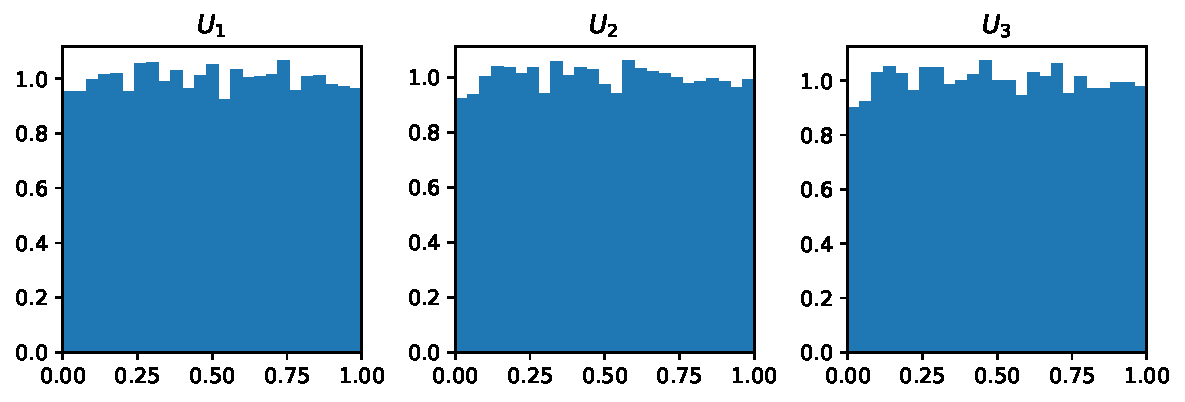
\includegraphics[width=0.99\linewidth]{figures/ND examples/Gaussian 3x3 large s power uniforms.pdf}
        \caption{}
        \label{fig:Gaussian 3x3 large s power uniforms}
    \end{figure}
    The resulting $u_i^{(j)}$ now seem to follow a uniform distribution and indeed the KDE fits much better as seen in \autoref{fig:Gaussian 3x3 large s power X3 KDE}.
    \begin{figure}[H]
        \centering
        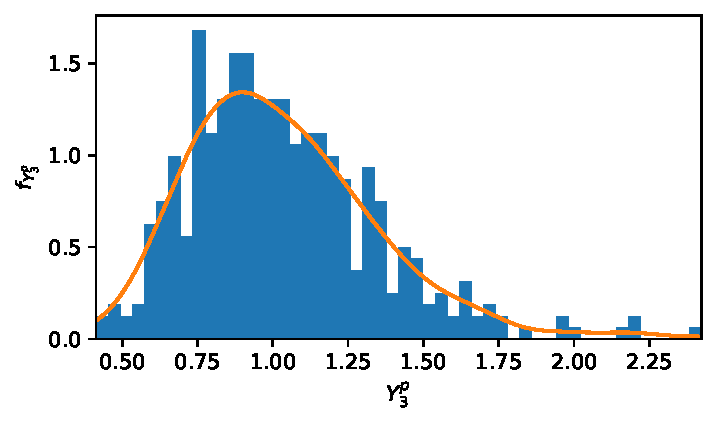
\includegraphics[width=0.7\linewidth]{figures/ND examples/Gaussian 3x3 large s power X3 KDE.pdf}
        \caption{}
        \label{fig:Gaussian 3x3 large s power X3 KDE}
    \end{figure}
    Turning to \autoref{alg:Gobs1} and \autoref{alg:ND} we now find that $G_{dir}$ is given by
    $$G_{dir} =
        \begin{bmatrix}
            -0.3290  & 0.6610   & 0.008440   \\
            0.6610   & -0.3290  & 0.008150   \\
            0.008440 & 0.008150 & -0.0002061
        \end{bmatrix}
    $$
    Which is indeed much more comparable with the result from before in \autoref{eq:s medium G_dir} and \autoref{eq:s small G_dir}. The difference between $G_{dir}$ from $\boldsymbol Y$ and $\boldsymbol Y^p$ is clearly visible in \autoref{fig:Gaussian 3x3 large s G_dir differences} and also \autoref{fig:Gaussian 3x3 large s power} resembles the original correlation structure.
    \begin{figure}[H]
        \centering
        \begin{subfigure}[t]{0.49\textwidth}
            \centering
            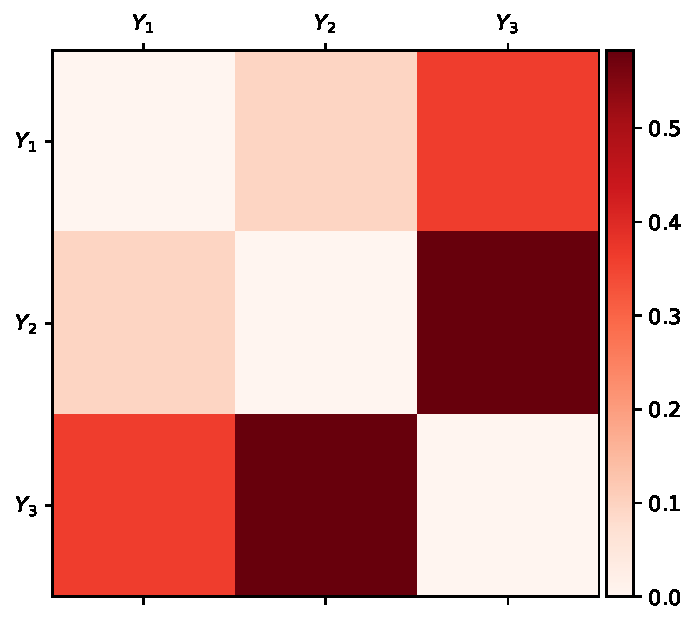
\includegraphics[width=\linewidth]{figures/ND examples/Gaussian 3x3 large s.pdf}
            \caption{}
            \label{fig:Gaussian 3x3 large s}
        \end{subfigure}%
        ~
        \begin{subfigure}[t]{0.49\textwidth}
            \centering
            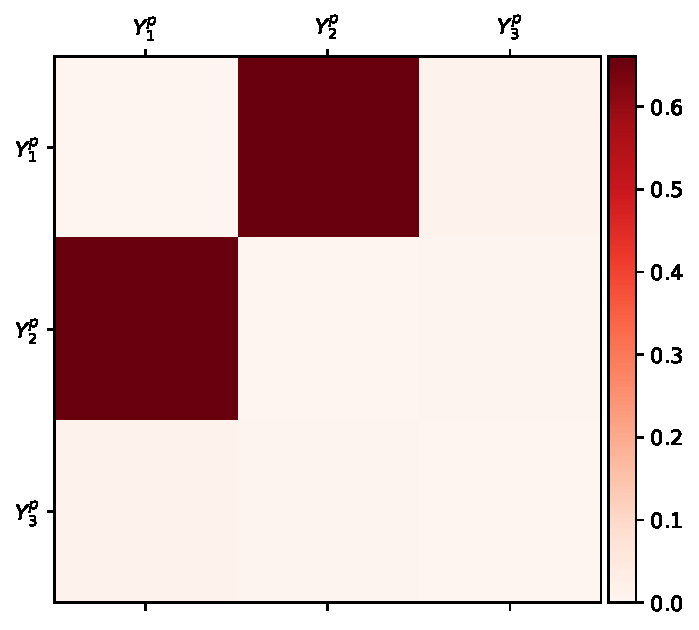
\includegraphics[width=\linewidth]{figures/ND examples/Gaussian 3x3 large s power.pdf}
            \caption{}
            \label{fig:Gaussian 3x3 large s power}
        \end{subfigure}
        \caption{$G_{dir}$ resulting from $10{,}000$ samples from multi variate Gaussian with $\boldsymbol\sigma = (1,2,3)$ in \textbf{(a)} with raw samples from $\boldsymbol Y$ and in \textbf{(b)} the transformed data corresponding to $\boldsymbol Y^p$.}
        \label{fig:Gaussian 3x3 large s G_dir differences}
    \end{figure}
    Finally, to end this example we shall compare with some theoretical results. Namely, the output $G_{obs}$ of \autoref{alg:Gobs1} can also be calculated theoretically. For this, we shall use \autoref{prop:MI bivariate gaussian} which permits a theoretical result, namely
    \begin{align*}
        G_{obs} & =
        \begin{bmatrix}
            0                                              & -\frac{1}{2} \ln \left( 1 - \rho_{12}^2\right) & -\frac{1}{2} \ln \left( 1 - \rho_{13}^2\right) \\
            -\frac{1}{2} \ln \left( 1 - \rho_{21}^2\right) & 0                                              & -\frac{1}{2} \ln \left( 1 - \rho_{23}^2\right) \\
            -\frac{1}{2} \ln \left( 1 - \rho_{31}^2\right) & -\frac{1}{2} \ln \left( 1 - \rho_{32}^2\right) & 0
        \end{bmatrix} \\
                & \cong
        \begin{bmatrix}
            0       & 0.83037 & 0 \\
            0.83037 & 0       & 0 \\
            0       & 0       & 0
        \end{bmatrix}
    \end{align*}
    Similarly, prior to deconvolution, using just the sampled $\boldsymbol X$ (i.e. no exponential transform), \autoref{alg:Gobs1} returns
    $$G_{obs} =
        \begin{bmatrix}
            0.         & 0.71841756 & 0.01781815 \\
            0.71841756 & 0.         & 0.01769672 \\
            0.01781815 & 0.01769672 & 0.
        \end{bmatrix}
    $$
    Clearly these are not equal, but in this case, the error is suspected to originate from the estimated joint density. For example, considering $X_1$ and $X_2$, we compare the estimated joint copula density and compare to the theoretical \textcolor{red}{reference til et sted hvor gausisk copula står} shown in \autoref{fig:gaussian copula estimate} and \autoref{fig:gaussian copula truth} respectively.
    \begin{figure}[H]
        \centering
        \begin{subfigure}[t]{0.45\linewidth}
            \centering
            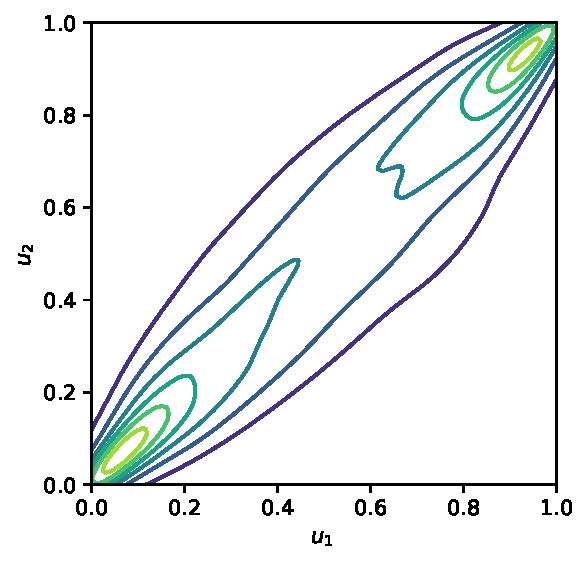
\includegraphics[width = \linewidth]{figures/ND examples/Gaussian copula sample contour.pdf}
            \caption{}
        \end{subfigure}%
        ~
        \begin{subfigure}[t]{0.5\linewidth}
            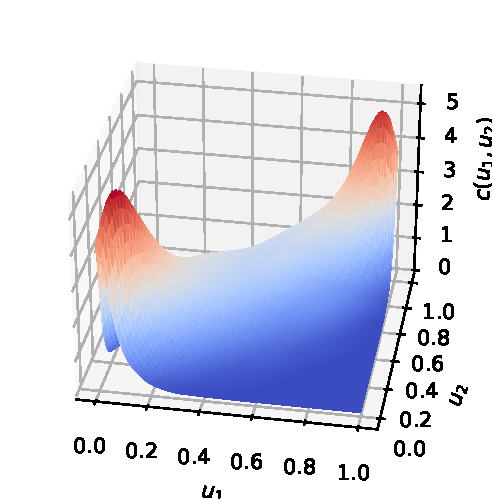
\includegraphics[width = \linewidth]{figures/ND examples/Gaussian copula sample pdf.pdf}
            \caption{}
        \end{subfigure}
        \caption{Estimated copula density $c$ with $\rho = 0.9$ corresponding to $X_1$ and $X_2$.}
        \label{fig:gaussian copula estimate}
    \end{figure}
    The noticeable difference is in the corners $(0,0)$ and $(1,1)$ where the theoretical copula density tends to infinity whereas the estimated density has modes at $(0.1,0.1)$ and $(0.9,0.9)$. In particular, simply rescaling the copula density in \autoref{alg:Gobs1} does not resemble the theoretical boundary which is a known issue \textcolor{red}{reference til artikel om undershoot peaks og boundary conditions for KDE}. A better approach may be to use jackknifing \textcolor{red}{link til afsnit of jackknifing, som også indeholder reference til artikel hvor dette gøres}.
    \begin{figure}[H]
        \centering
        \begin{subfigure}[t]{0.45\linewidth}
            \centering
            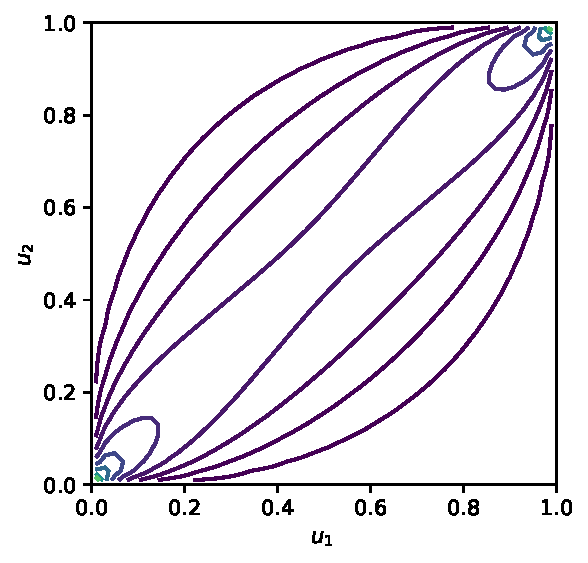
\includegraphics[width = \linewidth]{figures/ND examples/Gaussian copula theoretical contour.pdf}
            \caption{}
        \end{subfigure}%
        ~
        \begin{subfigure}[t]{0.5\linewidth}
            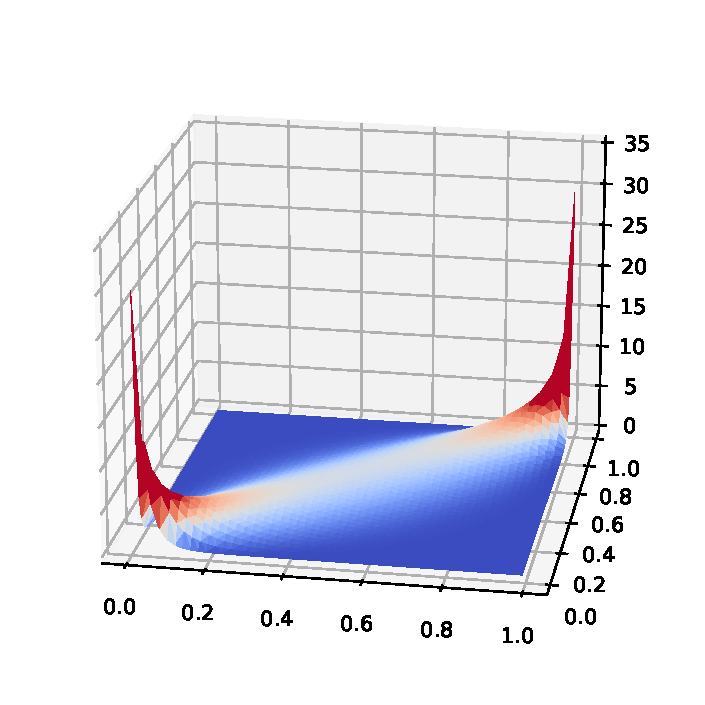
\includegraphics[width = \linewidth]{figures/ND examples/Gaussian copula theoretical pdf.pdf}
            \caption{}
        \end{subfigure}
        \caption{Theoretical copula density $c$ with $\rho = 0.9$ corresponding to $X_1$ and $X_2$.}
        \label{fig:gaussian copula truth}
    \end{figure}
    We note however, that the underlying structure is still captured i.e. that $Y_1$ and $Y_2$ covary while $Y_3$ does not inform $Y_1$ or $Y_2$ and vice versa.
\end{example}

We continue with a similar example to the previous one. The key difference is the number of variables and a more complicated correlation structure to test the algorithms further.
\begin{example}
    From \autoref{ex:1} we saw how one could handle some numerical issues. Thus, in this example we shall not bother ourselves with such computations and merely focus on the correlation structure. In particular, we shall sample $\boldsymbol X$ from a 10 dimensional
\end{example}


\newpage
\begin{proposition} \label{prop:MI bivariate gaussian}
    Given a bivariate normal distribution $\boldsymbol X \sim \mathcal{N}\left(\boldsymbol \mu,  \Sigma\right)$ where
    $$\Sigma =
        \begin{bmatrix}
            \sigma_1^2             & \rho \sigma_1 \sigma^2 \\
            \rho \sigma_1 \sigma_2 & \sigma_2^2
        \end{bmatrix}
    $$
    Then the mutual information $I\left(X_1, X_2\right) = -\frac{1}{2}\ln \left(1 - \rho^2\right)$.
\end{proposition}
\begin{proof}

\end{proof}

\end{document}










